\documentclass[12pt, titlepage]{article}

\usepackage{booktabs}
\usepackage{tabularx}
\usepackage{hyperref}
\usepackage{enumitem}
\usepackage{graphicx}
\hypersetup{
    colorlinks,
    citecolor=black,
    filecolor=black,
    linkcolor=red,
    urlcolor=blue
}
\usepackage[round]{natbib}

\title{SE 3XA3: Development Plan\\Title of Project}  % title of your project should go here

\author{Team \#, Team 3  % only need your team number once
		\\ Joel Straatman - straatjc
		\\ Nik Novak - novakn
		\\ Erin Varey - vareye
}

\date{\today}

%% Comments

\usepackage{color}

\newif\ifcomments\commentstrue

\ifcomments
\newcommand{\authornote}[3]{\textcolor{#1}{[#3 ---#2]}}
\newcommand{\todo}[1]{\textcolor{red}{[TODO: #1]}}
\else
\newcommand{\authornote}[3]{}
\newcommand{\todo}[1]{}
\fi

\newcommand{\wss}[1]{\authornote{blue}{SS}{#1}}
\newcommand{\ds}[1]{\authornote{red}{DS}{#1}}
\newcommand{\mj}[1]{\authornote{red}{MSN}{#1}}
\newcommand{\cm}[1]{\authornote{red}{CM}{#1}}
\newcommand{\mh}[1]{\authornote{red}{MH}{#1}}

% team members should be added for each team, like the following
% all comments left by the TAs or the instructor should be addressed
% by a corresponding comment from the Team

\newcommand{\tm}[1]{\authornote{magenta}{Team}{#1}}


\begin{document}

\maketitle

\pagenumbering{roman}
\tableofcontents
\listoftables
\listoffigures

\begin{table}[bp]
\caption{\bf Revision History}
\begin{tabularx}{\textwidth}{p{3cm}p{2cm}X}
\toprule {\bf Date} & {\bf Version} & {\bf Notes}\\
\midrule
October 7 & 1.0 &  Erin and Joel's sections\\
Date 2 & 1.1 & Notes\\
\bottomrule
\end{tabularx}
\end{table}

\newpage

\pagenumbering{arabic}

This document describes the requirements for Rather. The template for the Software
Requirements Specification (SRS) is a subset of the Volere
template~\citep{RobertsonAndRobertson2012}.  If you make further modifications
to the template, you should explicity state what modifications were made.

\section{Project Drivers}

\subsection{The Purpose of the Project}
The purpose of the project is to revise an already existing extension for Google Chrome which acts as a text-to-image replacement tool. The revised version will be more versatile, robust, and functional. The program's functionality will be expanded to most forms of social media, while simutaneously being more user friendly and dependable. 

\subsection{The Stakeholders}

\subsubsection{The Client}
The client is Dr. Spencer Smith at Mcmaster University and the marking ta's for 3xa3. % "ta" should be capitalized

\subsubsection{The Customers}
The client is anyone who uses Google Chrome and wishes to filter out unwanted things from their newsfeeds. The websites the filter currently works for are Twitter and Facebook

\subsubsection{Other Stakeholders}
% "stakeholders" does not need an apostrophe
The additional Stakeholder's in this project are anyone else who wishes to participate in the public project. This could include the original creator of Rather and anyone who finds the Git repository online. 

\subsection{Mandated Constraints}
The project must respect user privacy; refrain from recording or storing any data from the user's social media feeds. Even if this is not done with malicious intent, it is wise to avoid this practice to ensure there is nothing contentious about the program.

\subsection{Naming Conventions and Terminology}
The project will use a common naming convention for all files, functions, variables and constants. Files will be formally named with underscores instead of spaces. Functions will have no spaces, the first word is not capitalized, and all subsequent words are capitalized. Variables have no spaces, with all words capitalized. Constants are written in all capital letters. A Hash Tag is an image tag that is used to describe what an image is. For instance an image of someone's dog would be tagged dog. This is the only industry terminology referenced in this document.  

\subsection{Relevant Facts and Assumptions}
User must be able to read, use a computer, and have a Facebook and/or Twitter account. User must also have Google Chrome installed, and have a basic understanding of how extensions work for said browser.

User characteristics should go under assumptions. % you don't need this sentence from the original template

\section{Functional Requirements}


\subsection{The Scope of the Work and the Product}
The project will operate exclusively on Google Chrome, more specifically the sites Twitter and Facebook. The filtering is based on text that is read and it will not work for videos or images without text or tags. The search will only occur on Instagram. The code will be tested using Q-unit a Javascript package that allows unit testing.

\subsubsection{The Context of the Work}
Rather will operate under the assumptions that users have a fundamental basis in computer usage. It will also operate on the basis of users being familiar with Google Chrome and Google Chrome Extensions. The user will also have to be on either Facebook and Twitter for Rather to work, and ideally (not required) be familiar with Facebook and Twitter. The application will follow thecontrol flow diagram shown below:
\begin{figure}
  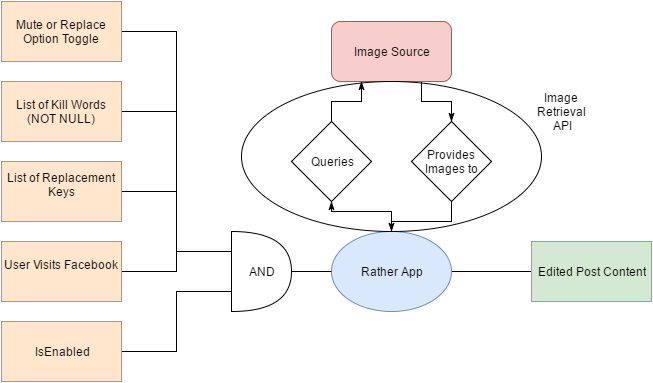
\includegraphics[width=\linewidth]{Rather_Control_Flow.png}
  \caption{Program Control Flow and Context}
  \label{fig:Control Flow Diagram}
\end{figure}


\subsubsection{Work Partitioning}
Work will be partitioned according to \href{../DevelopmentPlan/Dev_Plan_Rev0.gan}{Gantt chart}. All project milestones and division of labour wills tay up to date in the chart.

\subsubsection{Individual Product Use Cases}
\begin{itemize}
  \item A user encounters an annoying social media trend that is inhibiting their experience, or overwhelming their social media content. The user uses rather to remove these posts.
  \item A user suffering from PTSD is afraid to engage in social media due to images that may trigger unwanted memories. The user uses rather to replace undesirable content with soothing images.
  \item A user wishes to remain friends with another social media user, however does not like the content they post. Rather is used to remove the indesirable person's content from their feed, effectively ignoring the person in ana % typo here
   undetectable manner.
  \item A user is bored and wishes to replace as many posts on his feed with cats as possible.
  
\end{itemize}

\subsection{Functional Requirements}
\begin{itemize}
  \item The program shall take as input a set of key words specified by the user, known as a kill list. The user may specify multiple kill lists.
  \item The program shall likewise take as input from the user a set of words defining replacement content, known as replacement keys.
  \item The program shall take as input from the user an option to either mute or replace post content
  \item The program shall be able to identify individual posts on both Facebook and Instagram, and will only be active when the user visits these sites.
  \item The program shall perform a search for key words found both in the displayed text of the post as well as in any tags within the post's context to determine related content. The search shall encompass all of the user's posts visually displayed on the social media site.
  \item After a post containing a keyword is found, the program will be able to identify any images within the post.
  \item Depending on the user's preference of mute or replace, all images and text within the post's context will be either removed from view or replaced by images defined by replacement keys respectively.
  \item The program shall allow the user to undo any changes to individual posts without requiring a refresh.
\end{itemize}

\section{Non-functional Requirements}

\subsection{Look and Feel Requirements}
Rather is intended to have a sleek feel with the removed images. This means when an image is replaced with a more desirable image it should be approximately the same size as the original. This will prevent the image from appearing stretched or squashed and not looking aesthetically pleasing. Rather will be written so that the images do not take a long time to buffer. This will prevent loading images from freezing the user's computer and putting the unsightely loading screen as its replacement. 

\subsection{Usability and Humanity Requirements}
The user needs to have a computer with Google Chrome installed. The user needs to either be able to have vision or have some software that will read the application options to them. The user needs to have social media accounts where they follow people for the application to have images to replace. The program must save the user's defined kill lists in order to make use of the program in the future easier. If the program encounters an error, it will disable itself such that the user's content is not undesirably altered.

\subsection{Performance Requirements}
Rather should complete image replacement in under T seconds. It should not freeze the user's browser. T may vary depending on the user's system, however T must be less than or equal to the average load time of the initial page the program is operating on.
\subsection{Operational and Environmental Requirements}
The user should have the necessary computer input devices. This includes a mouse or keyboard. The user needs an environment with WIFI where they are able to operate a computer.

\subsection{Maintainability and Support Requirements}
Rather will be written in a way such that as long as there are not major changes in the source code of Facebook or Twitter the application will still function as expected. The developers will not maintain support for this application after the course is completed.

\subsection{Security Requirements}
The developers will not collect or store the user's information from social media. The developer's will not use malware or virus's % plural form of "virus" is "viruses"
in the application. There will not be a limit to what the user can filter. They are responsible for ensuring they are using appropriate replacement tags. 

\subsection{Cultural Requirements}
Rather is not responsible for the choice of replacement image used. It is the user's responsibility to ensure they are respecting other cultures with their replacement images.

\subsection{Legal Requirements}
Rather will only collect publically shared images. They do not own any images used. 

\subsection{Health and Safety Requirements}
The user is responsible for using correct form well operating their computer. It is not Rather's responsibility for any mistagged images. If the user experiences emotional distress from seeing an improperly tagged image Rather is not responsible. 

This section is not in the original Volere template, but health and safety are
issues that should be considered for every engineering project.

\section{Project Issues}

\subsection{Open Issues}
There are not currently any issues with the project repository. The orignal repository has two open issues that have not been addressed. The request for meme filter will not be addressed. The addition of an optional filter by name on Facebook/Twitter the group will attempt to implement. 

\subsection{Off-the-Shelf Solutions}
A potential solution is that name can be identified in the source code. The filter function can have a if option to skip certain names.

\subsection{New Problems}
The application no longer works for Facebook. This issue will be resolved in the new version. There is also an identity risk with use of the app, as it can be used to inaccurately represent a person in terms of the content that they are posting.

\subsection{Tasks}

\subsection{Migration to the New Product}
The new product will operate the same as the original. If the new feature is added the user will recieve an update blurb with an explanation on how to operate it. 

\subsection{Risks}
There are no risk associated with developing this.

\subsection{Costs}
There are no cost associated with this project aside from electricity used to work on this on our computers, and time. 

\subsection{User Documentation and Training}
There is a brief explanation blurb when the user installs rather. The application has subtitles that allow the user to find their block list and replacement list without having to re-read the blurb. No training is required.

\subsection{Waiting Room}
There are no requirements for future versions to be implemented.

\section{Appendix}
% This sentence from the template can be removed
This section has been added to the Volere template.  This is where you can place
additional information.

\subsection{Symbolic Parameters}
% This sentence from the template can be removed
The definition of the requirements will likely call for SYMBOLIC\_CONSTANTS.
Their values are defined in this section for easy maintenance.


\end{document}e